\documentclass[tikz,border=2pt]{standalone}
% Preámbulo común de los diagramas TikZ (misma paleta y letra que las notas)
\usepackage[T1]{fontenc}\usepackage[utf8]{inputenc}
\usepackage{libertinus}\usepackage{libertinust1math}
\usepackage[defaultsans,scale=0.92]{lato}
\usepackage{amsmath,amssymb,bm}
\usepackage{tikz}\usetikzlibrary{calc,positioning,arrows.meta,shapes.geometric,decorations.pathreplacing,decorations.pathmorphing,fit,backgrounds}
\definecolor{snlazul}{HTML}{1E5AA8}\definecolor{snlnoche}{HTML}{14213D}\definecolor{snlvioleta}{HTML}{6C4AB6}
\definecolor{snlcoral}{HTML}{D1495B}\definecolor{snlambar}{HTML}{E09F3E}\definecolor{snlverde}{HTML}{2A9D8F}
\definecolor{snlteal}{HTML}{0F7173}\definecolor{snlgris}{HTML}{5C677D}\definecolor{snlfondo}{HTML}{F4F6FA}
\tikzset{>={Stealth[length=2.2mm]},
  bloque/.style={draw=#1,fill=#1!8,thick,rounded corners=2pt,minimum height=11mm,minimum width=20mm,align=center,font=\small},
  bloque/.default=snlazul,
  suma/.style={draw=snlnoche,thick,circle,inner sep=0pt,minimum size=5mm},
  flecha/.style={->,thick,draw=snlnoche},
  etq/.style={font=\small,text=snlnoche},
  nota/.style={font=\footnotesize\sffamily,text=snlgris,align=center}}

\begin{document}
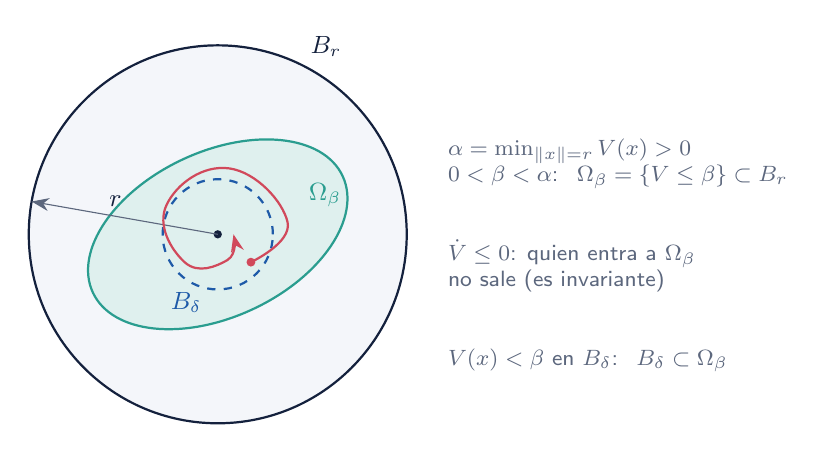
\begin{tikzpicture}
 \fill[snlfondo] (0,0) circle (2.4);
 \draw[snlnoche,thick] (0,0) circle (2.4);
 \node[etq] at (60:2.75) {$B_r$};
 \fill[snlverde!15,rotate=25] (0,0) ellipse (1.75 and 1.05);
 \draw[snlverde,thick,rotate=25] (0,0) ellipse (1.75 and 1.05);
 \node[etq,text=snlverde] at (20:1.45) {$\Omega_\beta$};
 \draw[snlazul,thick,dashed] (0,0) circle (0.7);
 \node[etq,text=snlazul] at (245:0.95) {$B_\delta$};
 \fill[snlnoche] (0,0) circle (1.5pt);
 \draw[snlgris,->] (0,0) -- (170:2.4) node[pos=0.55,above,etq]{$r$};
 \fill[snlcoral] (-40:0.55) circle (1.6pt);
 \draw[snlcoral,thick,->] plot[smooth,tension=0.8] coordinates {(-40:0.55) (10:0.9) (80:0.85) (150:0.75) (220:0.55) (290:0.35) (0:0.2)};
 \node[nota,align=left,anchor=west] at (2.8,0.9) {$\alpha=\min_{\|x\|=r}V(x)>0$\\ $0<\beta<\alpha$: \ $\Omega_\beta=\{V\le\beta\}\subset B_r$};
 \node[nota,align=left,anchor=west] at (2.8,-0.4) {$\dot V\le0$: quien entra a $\Omega_\beta$\\ no sale (es invariante)};
 \node[nota,align=left,anchor=west] at (2.8,-1.6) {$V(x)<\beta$ en $B_\delta$: \ $B_\delta\subset\Omega_\beta$};
\end{tikzpicture}
\end{document}
